For the Hanoi network, optimal solutions could be determined using the
Bisection Search. First results show that the least sensitive point is
always located close to the water source. This can be explained by the large water flow
from the reservoir to the first nodes. A leakage event along a pipe with
higher flow will lead to a less significant pressure drop when compared to a
leak along a pipe with lower flow. As this fact is known to water utility
administrators, we assume in follow up experiments that these nodes close to
the reservoir might be subject to increased protection. We treat them as
inaccessible for the adversary and remove them from the search space. 
\begin{figure}[h]
\centering
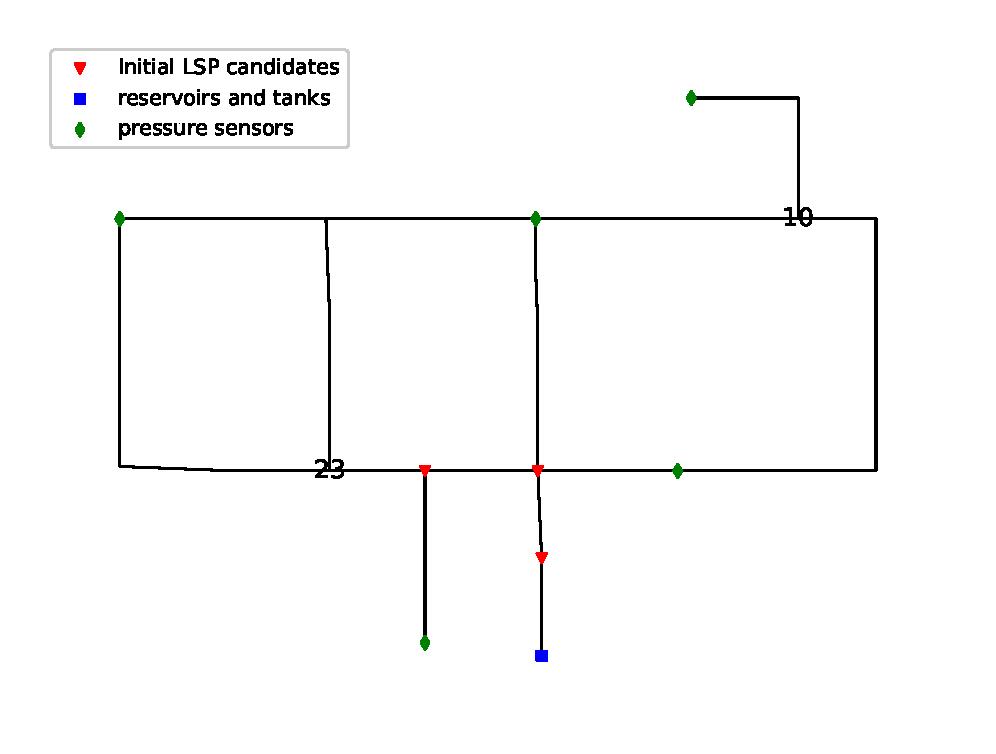
\includegraphics[height=0.3\textheight,width=\textwidth,keepaspectratio=True]{Figures/lsp_candidates_hanoi.eps}
\caption{Least Sensitive Point search on the Hanoi network: In initial
analysis, points with the lowest detector sensitivity (marked by red
triangles) are found close to the water reservoir. After excluding these
nodes from the search space, the least sensitive point is found at node 10
for the 2-days dataset and at node 23 for the 9-days dataset.
}
\label{fig:lsp_candidates_hanoi}
\end{figure}
In the 2-days dataset, the least sensitive point among the remaining nodes
is located at node 10. For the 9-days dataset, it is found to be node 23.
The results are visualized in Figure~\ref{fig:lsp_candidates_hanoi}.\\
To compare the performance between the Basic Genetic Algorithm and the extension with
spectral embeddings we run five trials of each algorithm for both datasets. In
all 20 cases, the respective algorithm is able to locate the least sensitive
point correctly. This demonstrates the high accuracy of both methods on
small water networks. In order to gain evidence for this assumption, a larger
number of trials could be conducted in future work.
